\documentclass[12pt]{article}
\setlength\parindent{0pt}
\usepackage{amsmath}
\usepackage{lscape}
\usepackage{graphicx}
\usepackage{color}
\usepackage{fullpage}
\usepackage[margin=0.8in]{geometry}
\setlength{\parskip}{4mm}
\def\LL{\left\langle}   % left angle bracket
\def\RR{\right\rangle}  % right angle bracket
\def\LP{\left(}         % left parenthesis
\def\RP{\right)}        % right parenthesis
\def\LB{\left\{}        % left curly bracket
\def\RB{\right\}}       % right curly bracket
\def\PAR#1#2{ {{\partial #1}\over{\partial #2}} }
\def\PARTWO#1#2{ {{\partial^2 #1}\over{\partial #2}^2} }
\def\PARTWOMIX#1#2#3{ {{\partial^2 #1}\over{\partial #2 \partial #3}} }
\newcommand{\BE}{\begin{displaymath}}
\newcommand{\EE}{\end{displaymath}}
\newcommand{\BI}{\begin{itemize}}
	\newcommand{\red}{\color{red}}
\newcommand{\EI}{\end{itemize}}
\newcommand{\BNE}{\begin{equation}}
\newcommand{\ENE}{\end{equation}}
\newcommand{\BEA}{\begin{eqnarray}}
\newcommand{\EEA}{\nonumber\end{eqnarray}}
\newcommand{\EL}{\nonumber\\}
\newcommand{\la}[1]{\label{#1}}
\newcommand{\ie}{{\em i.e.\ }}
\newcommand{\eg}{{\em e.\,g.\ }}
\newcommand{\cf}{cf.\ }
\newcommand{\etc}{etc.\ }
\newcommand{\Tr}{{\rm tr}}
\newcommand{\etal}{{\it et al.}}
\newcommand{\OL}[1]{\overline{#1}\ } % overline
\newcommand{\OLL}[1]{\overline{\overline{#1}}\ } % double overline
\newcommand{\OON}{\frac{1}{N}} % "one over N"
\newcommand{\OOX}[1]{\frac{1}{#1}} % "one over X"
\pagenumbering{gobble}
\begin{document}
\Large
\centerline{\sc{Tutorial-Exercise -- Kepler's Laws (instructor's guide)}}

\normalsize

In this exercise, you'll explore Kepler's laws of orbital motion.

Remember that these exercises are not meant for you to do alone; you should work with others near you on them, and should raise your hand and ask questions as you have them.

Your fourth homework assignment is included on the back of this handout. You should complete it by class time on October 12 (or 7) and put it in your TA's mailbox.

\bigskip\bigskip

\section{Kepler's First Law}

Kepler's first law says that planets orbit the Sun in an ellipse with the Sun at one {\it focus}. An ellipse has two foci; they lie along the long axis of an ellipse, are nearer the center for ellipses that are less eccentric (stretched out), and are nearer the edge for ellipses that are more eccentric (more stretched out).

Here are four orbits.

\begin{enumerate}
	\item Two of them have {\it two} possible locations for the Sun. Draw them in.
	\item One of them has only {\it one} possible location for the Sun. Draw it in.
	\item One of them is not a possible shape for a planet's orbit. Cross it out.
\end{enumerate}

\begin{minipage}{0.25\textwidth}
	\begin{center}
	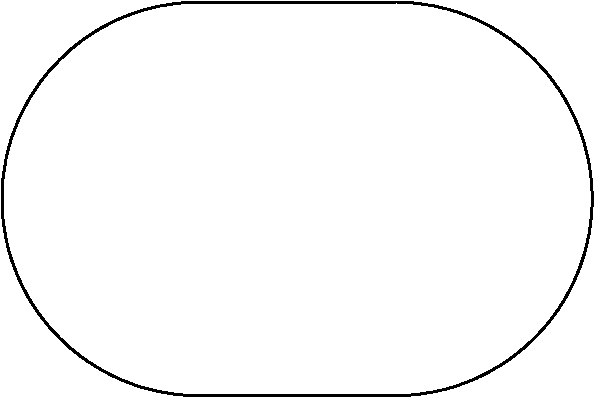
\includegraphics[width=0.9\textwidth]{oval-crop.pdf}
	\end{center}
\end{minipage}
\begin{minipage}{0.25\textwidth}
	\begin{center}
		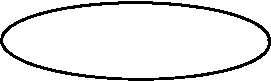
\includegraphics[width=0.9\textwidth]{highecc-crop.pdf}
	\end{center}
\end{minipage}
\begin{minipage}{0.25\textwidth}
	\begin{center}
		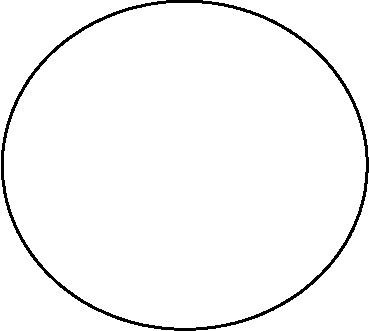
\includegraphics[width=0.9\textwidth]{lowecc-crop.pdf}
	\end{center}
\end{minipage}
\begin{minipage}{0.25\textwidth}
	\begin{center}
		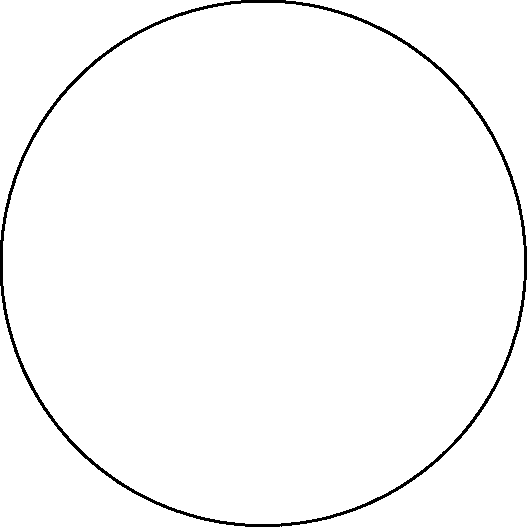
\includegraphics[width=0.9\textwidth]{circle-crop.pdf}
	\end{center}
\end{minipage}

{\color{red} The leftmost orbit isn't an ellipse; it's an oval. The second one is very eccentric, so its foci are close to the ends of the long axis. The third one is less eccentric, so its foci are closer to the center along the long axis. The rightmost one is a perfect circle; it has only one focus at the center.}

Of the three possible orbits, which one has zero eccentricity? 

{\red A circle is an ellipse with zero eccentricity, so that's the one on the right. Students may not realize at first that a circle is a special case of an ellipse.}


Which one has the highest eccentricity?

{\red The most stretched one (2).}

\newpage


\section{Kepler's Second Law}

As we saw demonstrated a bit ago, Kepler's second law says that an imaginary line between the Sun and a planet orbiting it sweeps out an equal amount of area in an equal amount of time. First, let's apply this to Earth's orbit, which is very close to a perfect circle.


Pretending for now that Earth's year is divided into twelve equal months and that its orbit is a perfect circle, here is a cartoon of Earth going around the Sun.
\begin{center}
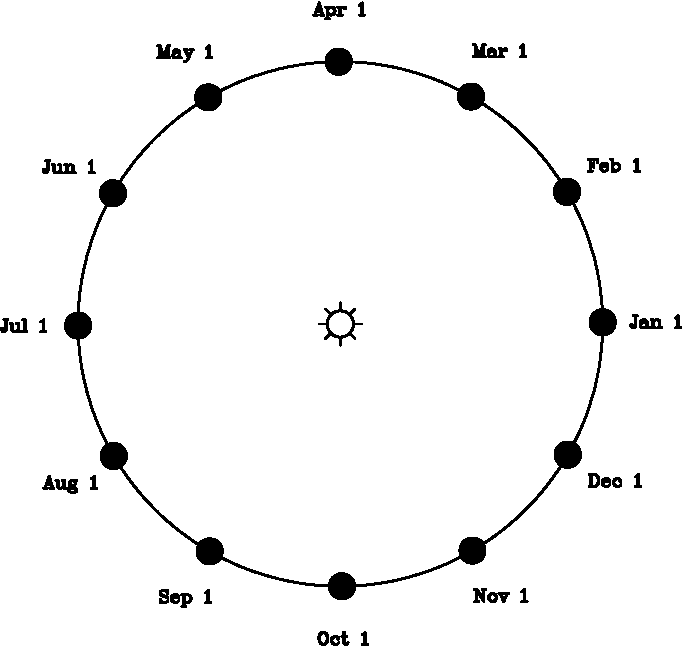
\includegraphics[width=0.4\textwidth]{earth-crop.pdf}
\end{center}
\begin{enumerate}
\item Using your pencil, shade the region that the imaginary line between Earth and the Sun sweeps out during January, and again during September. These regions should look like a piece of pizza with their point at the Sun.
{\red They will need to realize that the month of January goes from Jan 1 to Feb 1, and draw the appropriate pizza piece.}
\item Does Earth's orbit follow Kepler's second law? How do you know? 
{\red Each piece of pizza (area swept out by the line from Sun to Earth) is a month (equal time), and they all have equal area. Here the argument is trivial because of symmetry.}

{\color{blue} Here the idea is for students to get used to the argument -- this notion of equal-time-equal-area -- in a situation where symmetry makes it obvious.}


\item Kepler described his observations of planetary motion in terms of the ``area swept out'' by the line, but we can also think about the {\it speed} of Earth's motion.

Does the Earth move faster during January, move faster during September, or move at the same speed during both? How do you know? {\red The same during both -- Earth covers the same distance (1/12 of the way around its orbit, which we are treating as circular) in the same time (1 month). This is basically velocity equals distance over time, but without the formalism.}

\newpage

\item Now, let's consider a different planet whose orbit is more eccentric. 

Here is a cartoon of its orbit, showing its position at the beginning of January and February, along with several other positions

\begin{center}
	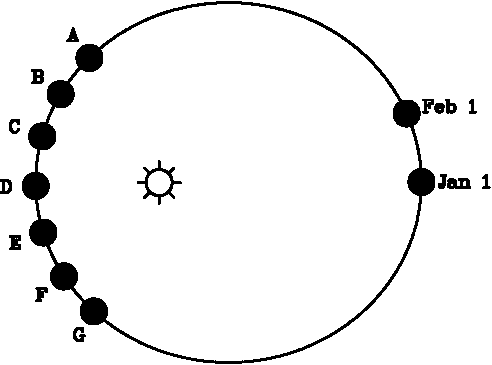
\includegraphics[width=3in]{pick-one-crop.pdf}
	
\end{center}


Shade in the area that the line connecting the Sun to the planet would sweep out during January, as you did before.

\bigskip

\item Then, find {\it two other} points in the orbit during which the line connecting the planet to the Sun would sweep out approximately that same area. You would like to fill in the blanks in the statement:


\bf ``As it moves from point \underline{\hspace{0.5in}} to point \underline{\hspace{0.5in}}, the line connecting this planet to the Sun sweeps out the same area as it does during the month of January.''

\rm


{\red This is the critical point here. The {\bf area} needs to match. It is not important what shape they draw over on the left -- we are not calculating things precisely -- but it should wind up spanning 4-6 letters. Many students -- particularly those who are used to the ``there is one right answer and I have to get someone to tell me what it is" mindset -- will have a tougher time thinking logically about this.}

Remember what ``area'' means: this means that if you were to color both areas in with ink, you would use the same amount of ink on both.

\bigskip

\item Does the motion on the left through the region you've highlighted take {\it more than}, {\it less than}, or {\it exactly} one month? How do you know? (Look back at the text of Kepler's second law on the front page.)

{\red People will try to overcomplicate this: it's exactly one month. Same area $\rightarrow$ same time. You may need to remind the students that Jan 1 to Feb 1 is one month.}

\vspace{1.5in}

\item Does the planet cover {\it more distance} during January or during the highlighted portion you've shown on the left?

{\red It will cover more distance during the highlighted portion close to the Sun. The cause-and-effect is important here: because the planet is closer to the Sun, it must travel further for the line connecting it to the Sun to sweep out the same area.}




\item {Does the planet {\it travel faster} during January or during the motion shown on the left? How do you know?}

{\red Again, we are doing velocity = distance / time, but without the formalism: to cover more distance in the same time, it must go faster.}




\item Now, let's think about the orbits of the planets known in Kepler's time. The eccentricity of Earth's orbit is 0.016. This is very small, so its orbit is very nearly circular. The orbits of Earth and the other inner planets look like this:

\begin{tabular}{|c|c|c|c|c|}
\hline
Planet & Perihelion (closest to Sun) & Aphelion (furthest from Sun) & Eccentricity \\ \hline
Mercury & 0.47 AU & 0.31 AU & 0.206 \\ \hline
Venus & 0.72 AU & 0.73 AU & 0.006\\ \hline
Earth &  0.98 AU & 1.02 AU & 0.016\\ \hline
Mars & 1.38 AU & 1.67 AU & 0.093 \\ \hline
\end{tabular}

Which of these planets {\it changes speed by the largest fraction} over the course of one orbit? How do you know?

{\red If they put together what they've just learned, then they can see that planets speed up when close to the Sun and slow down when they're further from it, and thus they're looking for the planet whose aphelion and perihelion are different by the greatest fraction. Helpfully I've calculated the eccentricity for them so they can just look at that: largest eccentricity = largest change, so Mercury.}

\vspace{1in}

\item Which of these planets {\it changes speed by the smallest fraction} over the course of one orbit? How do you know?

{\red Smallest eccentricity = smallest change, so Venus.}

\end{enumerate}

\section{Kepler's Third Law}

We'll be studying Kepler's third law in depth in lab -- not here.

The things you should know for now are only that:

\BI
\item Planets in larger orbits take longer to go around the Sun
\item The time it takes a planet to go around the Sun depends only on the long axis of its orbit; it does {\it not} depend on the planet's mass or size. (Jupiter takes longer to go around the Sun than Earth because it is further away, {\it not} because it is bigger.)
\EI

%Kepler's third law says that:
%
%\begin{center}
%	
%	\bf ``The square of the time that it takes a planet to go around the Sun is proportional to the cube of the long axis of its orbit.''
%\end{center}
%
%Translated into modern mathematics, we could also say:
%
%\begin{center}
%	
%	\bf ``The time it takes for a planet to go around the Sun is proportional to the 3/2 power of the long axis of its orbit.
%\end{center}
%
%We will do some more precise calculations based on this in lab. For now, you can just know:
%
%\begin{center}
%	\bf ``If a planet's distance from the Sun increases by some factor, its orbital period increases by {\it more} than that factor.''
%\end{center}
%
%
%
%
%	Earth is in a circular orbit around the Sun with a radius of about 1 AU, while Saturn is in a circular orbit with a radius of about 10 AU. Will Saturn take less than one year, between one and ten years, about ten years, or more than ten years to go around the Sun? How do you know?
%
%
%
%\newpage
%
%Here are some data on the planets:
%
%\begin{center}
%	
%	
%\begin{tabular}{|c|c|c|c|}
%	\hline
% & {\bf Orbital Distance} & {\bf Orbital Period} & {\bf Mass} \\
%	& (AU) & (years) & (Earths) \\ \hline
%	\bf Mercury & 0.38 & 0.24 & 0.06 \\ \hline
%	\bf Venus & 0.72 & 0.61 & 0.82 \\ \hline
%	\bf Earth & 1 & 1 & 1 \\ \hline
%	\bf Mars & 1.52 & 1.88 & 0.11 \\ \hline
%	\bf Jupiter & 5.20 & 11.86 & 318 \\ \hline
%	\bf Saturn & 9.54 & 29.46 & 95.2 \\ \hline
%\end{tabular}
%
%Notice that the planets have wildly varying masses: Jupiter is five thousand times more massive than Mercury.
%
%\end{center}
%
%	Based on these data and what you know about Kepler's third law, what is the relationship between the mass of a planet and how long it takes to orbit the Sun?
%	
%	\vspace{1.5in}
%	
%	If there {\it is} a relationship, describe where that relationship comes from. If there is {\it not} a relationship between mass and orbital period, discuss how the data from the table tell you that.
%	
%	\vspace{1.5in} 
%	
%	What is the dominant factor in determining how long it takes for a planet to go around the Sun?
%
%



\newpage

\begin{center}
	\sc \Large Homework 4 -- Kepler's Second Law
	
	\normalsize \it Due Tuesday, October 11. The quiz will be at the end of that class.
\end{center}

Suppose that a fictional planet that divides its years into twelve equal months has a pretty elliptical orbit. Astronomers on this planet are trying to figure out how it moves around its star during a year. They propose two options:

\bigskip

\begin{minipage}{0.5\textwidth}
	\begin{center}
		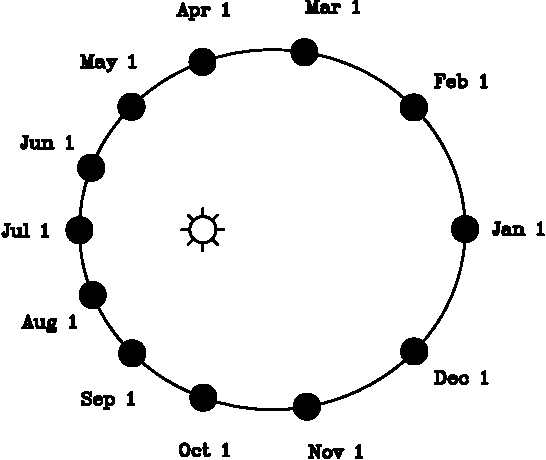
\includegraphics[width=0.6\textwidth]{choice2-crop.pdf}
		
		Choice A
	\end{center}
\end{minipage}
\begin{minipage}{0.5\textwidth}
	\begin{center}
		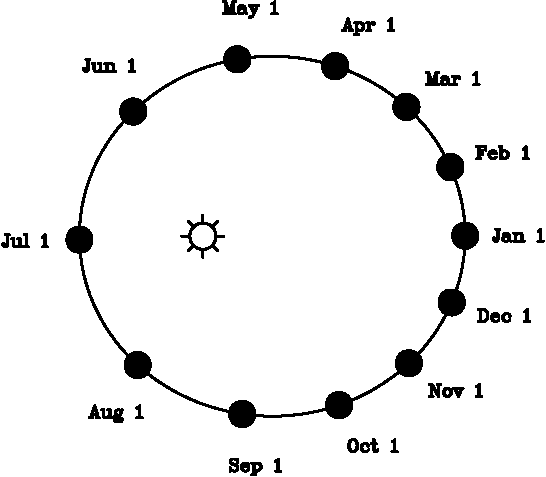
\includegraphics[width=0.6\textwidth]{choice1-crop.pdf}
		
		Choice B
	\end{center}
\end{minipage}


Three astronomers -- Alex, Bethany, and Chen -- are debating which one is correct.


{\bf Alex:} I think Choice A is correct. The planet is supposed to go fastest when it is near the Sun, right? So the months are spaced closer there since it is going faster.

{\bf Bethany:} Yes it is. But Choice B shows an orbit where the planet is moving slowly far away from the Sun, since it covers less distance each month.

{\bf Chen:} I think neither one can be right. The months are supposed to be equally-spaced and last the same amount of time, right? So the dots should be equally far apart, since the orbit is one year, and the months are equal portions of that. So you should draw another diagram like that.
\begin{enumerate}	

\item Who is correct? Write a few sentences explaining why and how you know.


\vspace{3in}

\item Is the planet moving faster in July or January? How do you know?


\vspace{1.5in}

\item Is the planet speeding up or slowing down in April? How do you know?

\vspace{1.5in}
	
\end{enumerate}

\begin{center}\underline{\hspace{3in}}\end{center}

The quiz on this material will be on Tuesday, October 11, and will consist of two questions.

\begin{enumerate}
	\item On the first question, I will ask you to draw a possible orbit for a planet around a star that meets certain criteria.
	
	\item On the second question, I will draw the orbit of a planet around its star for you, and then ask you questions about the planet's motion in that orbit.
\end{enumerate}

	
\end{document}




